\subsection{Présentation}

Les agents peuvent porter et utiliser des objets, et ces objets modifient leurs caractéristiques physiques ou cognitives. Par exemple,utiliser une longue-vue augmente la vision, une arme la puissance de frappe, la nourriture permet d’augmenter l’énergie physique et de diminuer la faim, etc. 

Ces objets peuvent être de plusieurs types, et sont générés par les actions des agents. Ils peuvent être récoltés, comme c’est le cas pour les matières premières (céréales,gibier, bois, minerai, etc.) ou fabriqués à partir d’une recette. Une recette décrit simplement l’ensemble des composants (nature et quantité) dont un objet a besoin pour être créé, ainsi que du cogniton nécessaire à l’agent pour pouvoir le fabriquer (ex : une poterie nécessite de l’argile mais aussi le savoir-faire d’un potier).

La possession d’un objet, son utilisation ou sa destruction sont susceptibles de modifier les cognitons de l’agent (un outil favorise certaines qualités) comme ses attributs (accroissement ou perte d’énergie). Ainsi il est donc aisemment possible pour les agents de transmettre des connaissances (échange d'un objet apportant un cogniton) mais aussi de modéliser des phénomènes de renforcements (la création d'un objet améliore les compétences nécessaires pour recréer un même objet ).

\subsection{Création d'un objet}

La création d'un objet se fait au moyen de l'onglet d'édition d'objet inventaire accessible au moyen de l'icône 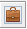
\includegraphics{images/item.png}.
Pour cela, une fois sur cet onglet, il suffit de cliquer sur l'icône 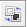
\includegraphics{images/create.png} pour qu'un nouvel objet soit créé avec pour nom Default\_ X. Cet objet est cependant vide de toutes caractéristiques, pour les spécifier il suffit de cliquer dessus. Vous obtiendrez ainsi, l'écran suivant : \newline

\begin{figure}[!h]
\begin{center}
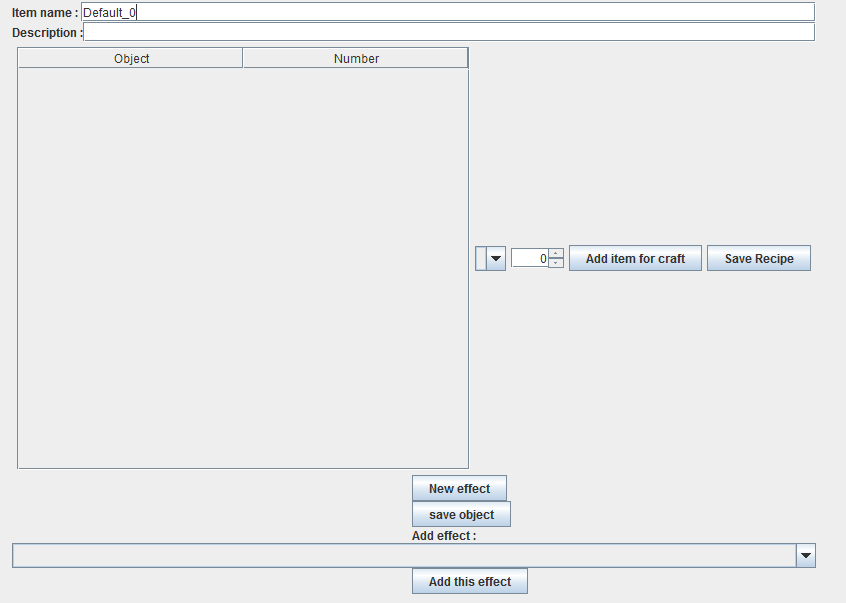
\includegraphics[scale = 0.7]{images/ecran.png}
\caption[eff]{Interface de création d'objet \\}
\label{Interface de création d'objet}
\end{center}
\end{figure}


Cet écran contient plusieurs parties permettant de définir l'objet.

Tout d'abord, les deux cases du haut permettent, comme leur nom l'indique, de spécifier le nom et la description de l'objet. 

Ensuite, le cadre contenant une colonne "Object" et une colonne "Number" correspond a la recette de création de l'objet, c'est a dire, les objets qui devront être détenus par l'agent lorsqu'il voudra fabriquer cet objet.
Pour ajouter un objet a la recette, il suffit de choisir le nom de l'objet à ajouter a la recette dans la liste déroulante située à la droite du cadre ainsi que le nombre d'unités de cet objet nécessaires à la recette. Les objets présents dans la liste déroulante sont les objets créés et sauvegardés précédemment. Il convient donc de créer en premier les ressources dites de base, a savoir, qui ne se fabriquent pas mais sont le résultat d'une récolte. Une fois les objets de la recette ajoutés il suffit de cliquer sur le bouton "Save Recipe" pour l'enregistrer.

Enfin, il faut maintenant définir les effets produits par l'objet sur son possesseur ou son utilisateur. Le bouton "New effect" permet de définir un nouvel effet a ajouter a l'objet. L'interface de création de cet effet apparait alors a droite du bouton "Save Recipe". \newline

\begin{figure}[!h]
\begin{center}
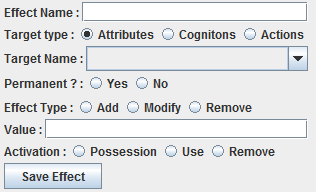
\includegraphics[scale = 1.0]{images/effets.png}
\caption[eff]{Interface de création d'effet \\}
\label{Interface de création d'effet}
\end{center}
\end{figure}

Après la spécification du nom, la sélection du "Target type" permet, comme son nom l'indique, de choisir la cible de l'effet, les attributs physiques de l'agent ou bien les cognitons constituant son esprit, la sélection de Actions permet de faire effectuer une action a l'agent. Il convient donc de définir les caractéristiques et l'agent ainsi que les cognitons constituant son esprit. Après avoir choisi le nom de l'attribut, du cogniton, ou de l'action ciblé par l'effet, le bouton "Permanent?" permet de définir si l'effet se terminera a la destruction de l'objet ou non. Ensuite la sélection du type de l'effet couplée au champ de texte "Value" permet de spécifier la valeur que l'on doit ajouter, retirer ou bien modifier a la valeur respectivement, de la caractéristique physique, du poids du cogniton défini lors de la sélection du "Target name". Enfin, on spécifie le cas d'activation de cet effet, a la possession, l'utilisation ou bien la destruction de l'objet en cours de définition. Il suffit enfin de cliquer sur le bouton "Save Effect" pour enregistrer l'effet en question.

Un autre moyen d'associer un effet a cet objet consiste a sélectionner le nom d'un effet précédemment enregistré dans la liste déroulante "Add effect" puis de cliquer sur le bouton "Add this effect" pour associer cet effet a l'objet.

Un objet peut ne pas avoir d'effet comme il peut ne pas avoir de recette. Seul le nom est obligatoire lors de la création d'un objet.

Une fois ces caractéristiques définies il suffit de cliquer sur le bouton "Save object" pour enregistrer l'objet dans la simulation.

\subsection{Observation durant la simulation}

Durant la simulation les objets portés par chaque agent peuvent être observés dans l'onglet "Agent". La colonne "Inventaire" contenant l'ensemble des objets portés par l'agent. Leurs différents effets peuvent être observés de façon indirecte en observant l'évolution des objets présents dans l'inventaire ainsi que les poids des cognitons et des plans présents dans l'esprit de l'agent et représentés dans ce même onglet.